\subsection{Confronto controllato con i metodi classici}

La campagna F1 confronta Fixed FEM, un monitor Winslow-type, un monitor arc-length, un monitor Hessian-based e GDM. Tutti i metodi mantengono 1089 nodi, 2048 triangoli e la connettività iniziale, con identici PDE, condizioni al contorno, griglia temporale, solver ALE e frequenza di adattamento. Le strategie classiche sono controller MMPDE-type a gradiente discreto; i monitor dipendono dal campo FEM numerico e sono aggiornati a ogni finestra. I parametri di intensità sono selezionati sulla validation tra quattro candidati per monitor. La Figura~\ref{fig:f1_alpha_validation} documenta la risposta dell'errore ai valori testati; griglia e conteggi degli eventi che raggiungono il limite iterativo sono riportati nell'Appendice~\ref{app:stageef}.



\begin{figure}[H]
\centering
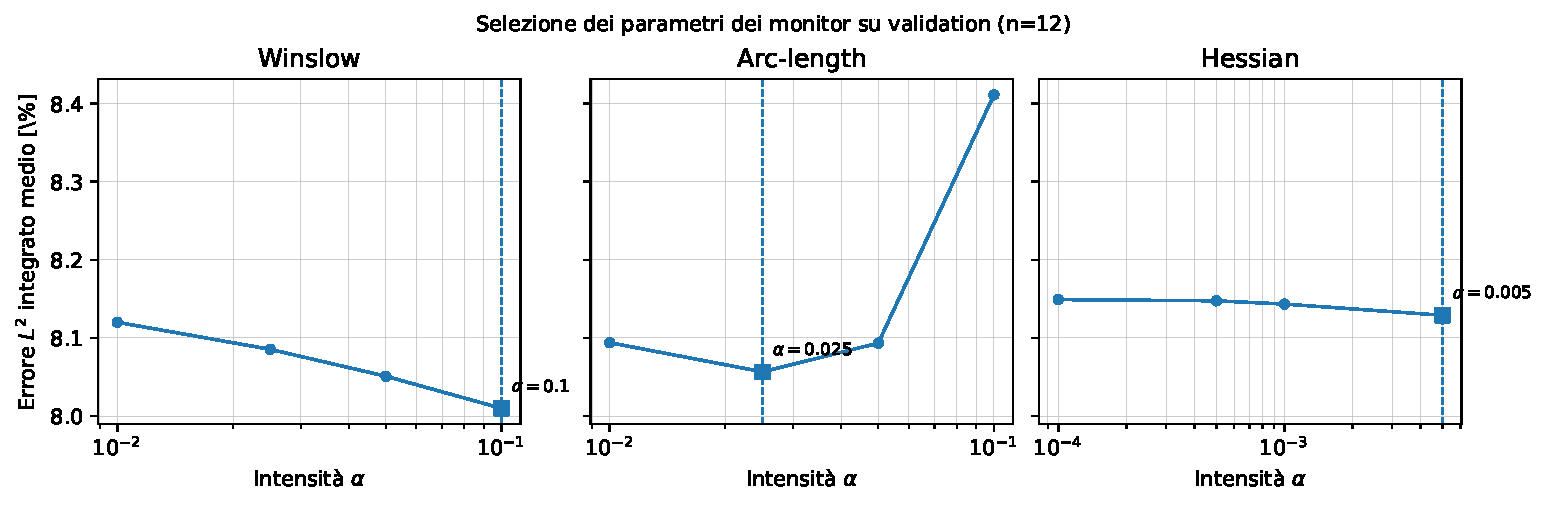
\includegraphics[width=\columnwidth,keepaspectratio]{images/stage_f/diagnostics/monitor_strength_validation.pdf}
\captionof{figure}{Errore integrato medio sui 12 casi validation in funzione dell'intensità del monitor; i marcatori indicano i valori selezionati.}
\label{fig:f1_alpha_validation}
\end{figure}

\subsection{Accuratezza sul test held-out}

L'endpoint primario è l'errore relativo $L^2$ medio nel tempo. La Tabella~\ref{tab:f1_errors} mostra che GDM ottiene la media più bassa sul totale e in entrambi gli split. La Tabella~\ref{tab:f1_paired} riporta le riduzioni relative appaiate, i relativi intervalli bootstrap e il numero di casi favorevoli. Tutti i 28 confronti hanno segno favorevole a GDM; il minimo $p$ grezzo esatto deriva da questa concordanza e non misura la grandezza dell'effetto. Il bootstrap ricampiona i casi e non la variabilità tra seed di addestramento; è stato valutato un solo checkpoint.

\begin{table*}[!t]
\centering\small
\caption{Errore relativo $L^2$ integrato medio per strategia e split nella campagna F1. Valori percentuali.}
\label{tab:f1_errors}
\begin{tabular*}{\textwidth}{@{\extracolsep{\fill}}lrrr}
\toprule
Strategia & Interpolazione ($n=12$) & Estrapolazione ($n=16$) & Totale ($n=28$)\\
\midrule
Fixed FEM & 8.729 & 12.060 & 10.633\\
Winslow-type & 8.575 & 11.696 & 10.358\\
Arc-length & 8.648 & 11.949 & 10.535\\
Hessian-based & 8.699 & 11.987 & 10.578\\
\textbf{GDM} & \textbf{8.043} & \textbf{11.172} & \textbf{9.831}\\
\bottomrule
\end{tabular*}
\end{table*}

\begin{table*}[!t]
\centering\small
\caption{Riduzione relativa media dell'errore integrato di GDM rispetto alle baseline sui 28 casi. IC bootstrap appaiato percentile al 95\%; $p$ corretto con Holm su 12 confronti.}
\label{tab:f1_paired}
\begin{tabular*}{\textwidth}{@{\extracolsep{\fill}}lrrrc}
\toprule
Baseline & Riduzione [\%] & IC 95\% [\%] & Casi favorevoli & $p_{\mathrm{Holm}}$\\
\midrule
Fixed FEM & 8.038 & [7.590, 8.506] & 28/28 & $8.94\times10^{-8}$\\
Winslow-type & 6.096 & [5.337, 6.859] & 28/28 & $8.94\times10^{-8}$\\
Arc-length & 6.981 & [6.653, 7.334] & 28/28 & $8.94\times10^{-8}$\\
Hessian-based & 7.805 & [7.197, 8.433] & 28/28 & $8.94\times10^{-8}$\\
\bottomrule
\end{tabular*}
\end{table*}

\subsection{Geometria e diagnostica del tracking}

La Tabella~\ref{tab:f1_geometry} riporta gli indicatori aggregati.

\begin{table*}[!t]
\centering\small
\caption{Diagnostiche geometriche aggregate sui 28 casi F1.}
\label{tab:f1_geometry}
\begin{tabular*}{\textwidth}{@{\extracolsep{\fill}}lrrrr}
\toprule
Strategia & $\min J$ & Media min. Escobar & Peggiore Escobar & Max aspect ratio\\
\midrule
Fixed FEM & $9.77\times10^{-4}$ & 0.866 & 0.866 & 1.394\\
Winslow-type & $7.81\times10^{-4}$ & 0.823 & 0.814 & 1.514\\
Arc-length & $8.03\times10^{-4}$ & 0.779 & 0.711 & 1.784\\
Hessian-based & $8.43\times10^{-4}$ & 0.835 & 0.819 & 1.503\\
GDM & $1.00\times10^{-4}$ & 0.398 & 0.324 & 4.016\\
\bottomrule
\end{tabular*}
\end{table*}

La diagnostica del tracking su quattro casi validation comprende 40 eventi e 404 snapshot. La densità relativa degli elementi nella corona $0.5\sigma\le r\le2\sigma$ ha mediana 1.213; il rapporto $h_{\mathrm{globale}}/h_{\mathrm{corona}}$ ha mediana 1.111. La distanza normalizzata tra centroide della concentrazione e centro gaussiano ha mediana $0.49\sigma$ sull'intera traiettoria e $0.61\sigma$ agli istanti finali: il tracking è quindi misurabile. La Figura~\ref{fig:f1_tracking_summary} riassume questa diagnostica; la Figura~\ref{fig:f1_tracking_case} mostra un caso rappresentativo.

\begin{figure}[H]
\centering
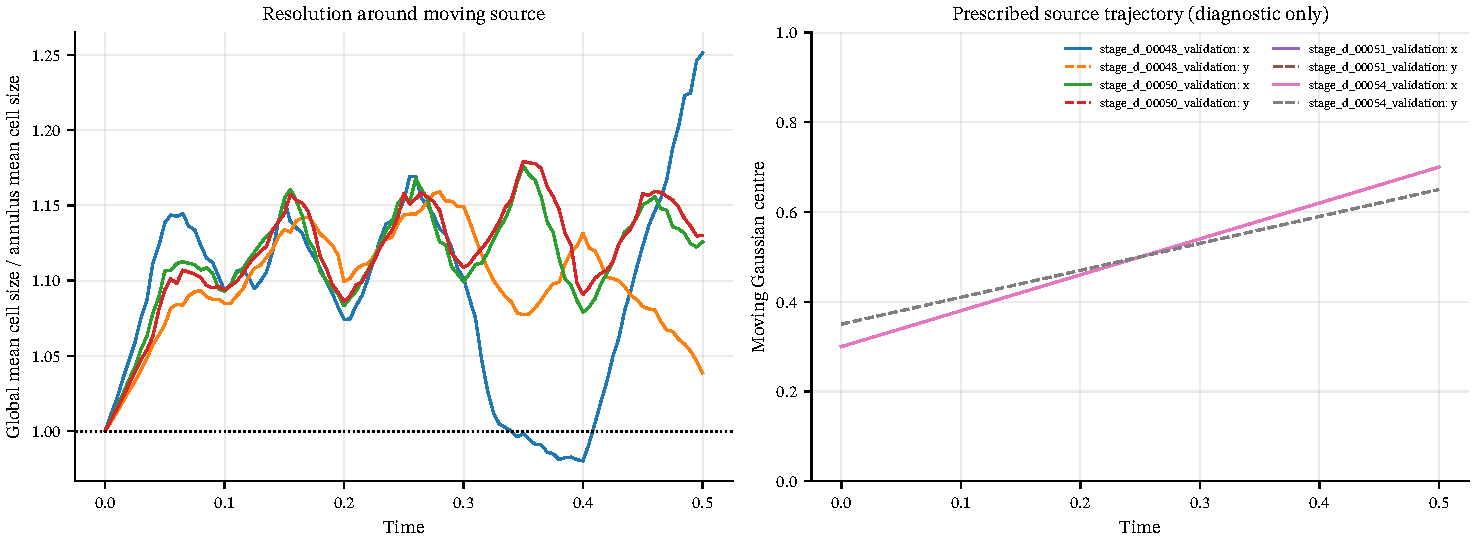
\includegraphics[width=\columnwidth,keepaspectratio]{images/stage_f/mesh_source_tracking_summary.pdf}
\caption{Tracking della regione gaussiana mobile su quattro casi validation: arricchimento locale della mesh e posizione del centroide della concentrazione.}
\label{fig:f1_tracking_summary}
\end{figure}

\begin{figure*}[!htbp]
\centering
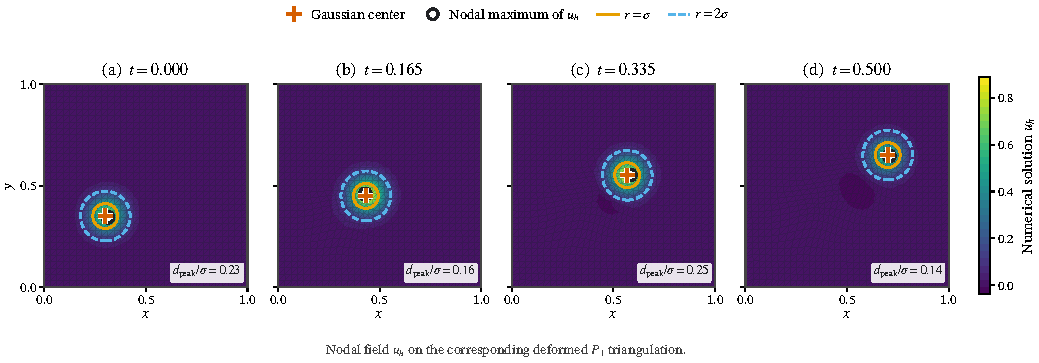
\includegraphics[width=1.0\textwidth,keepaspectratio]{images/stage_f/mesh_source_tracking_case_0054.pdf}
\caption{Evoluzione temporale della mesh e del campo numerico.}
\label{fig:f1_tracking_case}
\end{figure*}

\subsection{Filtro e costo online}

La Figura~\ref{fig:f1_safety_diagnostics} mostra la distribuzione dei fattori e le verifiche geometriche prima e dopo il filtro. I dati sono validation, non held-out test.

\begin{figure}[H]
\centering
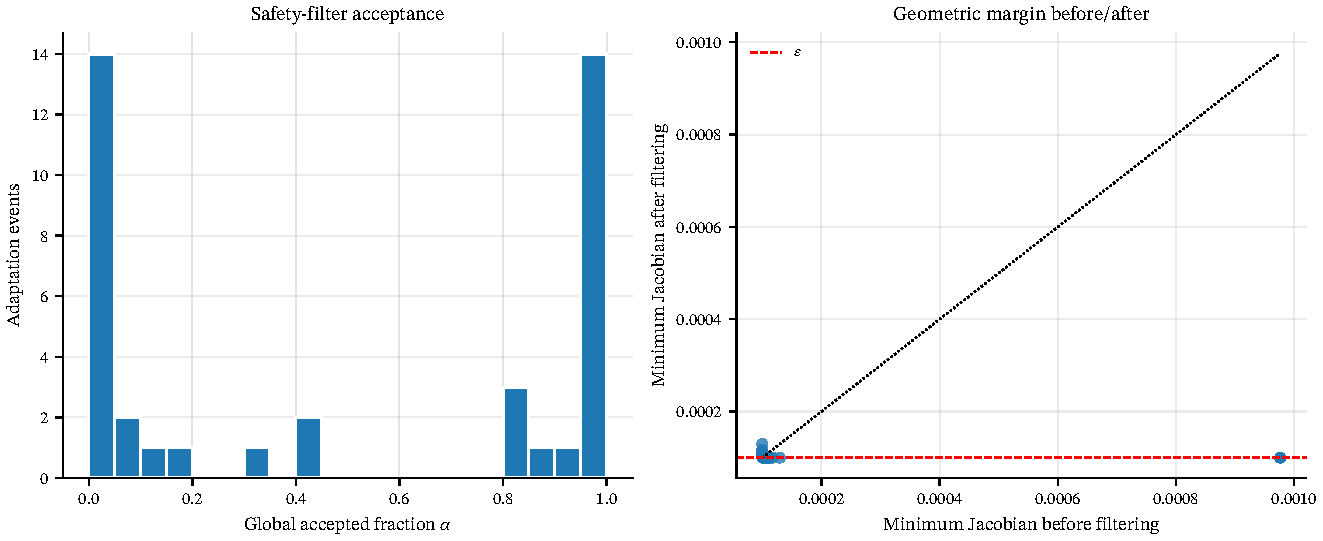
\includegraphics[width=\columnwidth,keepaspectratio]{images/stage_f/safety_filter_diagnostics.pdf}
\caption{Fattori globali $\alpha$ e diagnostiche geometriche raw/safe su 40 eventi validation.}
\label{fig:f1_safety_diagnostics}
\end{figure}

Il tempo online mediano per traiettoria è 0.117 s per Fixed FEM e 1.474 s per GDM (12.59 volte); i controller MMPDE richiedono 6.728--12.356 s. Questi tempi descrivono le implementazioni misurate.
\begin{table}[H]
\centering\small
\caption{Tempo online mediano per traiettoria F1; warm-up escluso e cinque ripetizioni per caso.}
\label{tab:f1_runtime}
\begin{tabular}{lrr}
\toprule
Strategia & Tempo [s] & Rapporto\\
\midrule
Fixed FEM & 0.117 & $1.00\times$\\
GDM & 1.474 & $12.59\times$\\
Arc-length & 6.728 & $57.49\times$\\
Hessian-based & 9.603 & $82.07\times$\\
Winslow-type & 12.356 & $105.58\times$\\
\bottomrule
\end{tabular}
\end{table}
